\chapter{Grundlagen von Spark}
\label{chapter:grundlagen von Spark}


Rund um Hadoop beziehungsweise Spark wurde in Berkeley ein ganzer Infrastruktur-Stack für Big-Data-Analytics aufgebaut, der BDAS.


\section{Der Berkeley Data Analytics Stack (BDAS)}
\label{section:der Berkeley Data Analytics Stack (BDAS)}

	
	Im Folgenden wird der Big Data Analytics Stack (BDAS) näher vorgestellt, der wie in der Einführung bereits erwähnt um Hadoop, bzw. Spark als Hauptbestandteile herum aufgebaut ist. Der BDAS wurde von den AMPLabs (kurz für „algorithms, machines and people“) von der University of California in Berkeley aufgrund von Forschungs-ergebnissen im Bereich der Analyse sehr großer Datenmengen ins Leben gerufen. 

Der Einsatz des BDAS kann laut Vijay Agneeswaran [VA14] dabei helfen, unter anderem Fragen wie die folgenden zu beantworten: 

\begin{itemize}
		\item Wie segmentiert man am besten eine Menge von Nutzern und kann herausfinden, welche Nutzersegmente an bestimmten Kampagnen interessiert sein könnten?
		\item Wie kann man richtige Metriken für Nutzer-Engagement in Social-Media-Applikationen herausfinden?
		\item Wie kann ein Video-Streaming-Dienst für jeden Nutzer dynamisch ein optimales Content-Delivery-Network (CDN) basierend auf Daten wie Bandbreite, Auslastung, Pufferrate, etc Auswählen?
		
\end{itemize}	


Prinzipiell sind die in der Einführung in Kürze beschriebenen Einschränkungen von Hadoop und die damit verbundene Motivation für Spark auch die Motivation für den BDAS. 


In Abbildung 2.1 wird eine Übersicht über die drei Hauptschichten des BDAS gezeigt. Rot dargestellt ist hier jeweils die von den AMPLabs empfohlene Implementierung.

\begin{figure}[htb!]
\centering
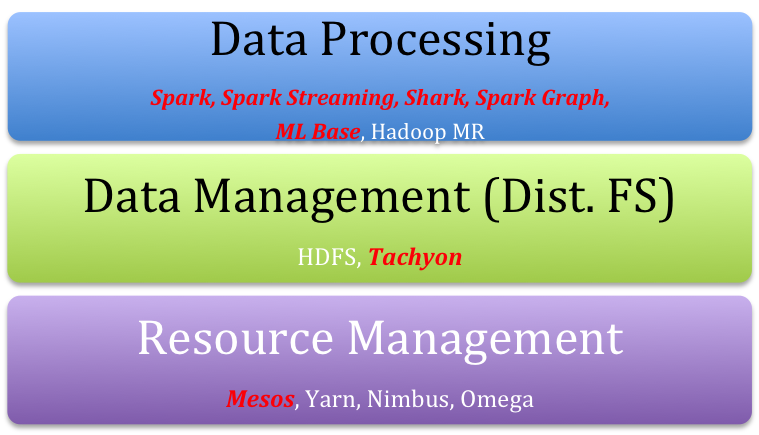
\includegraphics[width=1.0\textwidth]{bilder/2_1_stack.png}
\caption{Grobübersicht über den BDAS mit den drei Hauptschichten}
\label{fig:grobübersicht über den BDAS mit den drei Hauptschichten}
\end{figure}
 


In Abbildung 2.2 ist der Aufbau des BDAS nochmals schematisch dargestellt. Die grün hinterlegten Elemente markieren die Bestandteile des aktuellen BDAS, die violett hinterlegten zeigen alternative Implementierungen auf der jeweiligen Schicht. Grün schraffiert ist die Applikationsschicht, wo Applikationen oberhalb von Spark und den direkten Anwendungen angesiedelt sind. 

\begin{figure}[htb!]
\centering
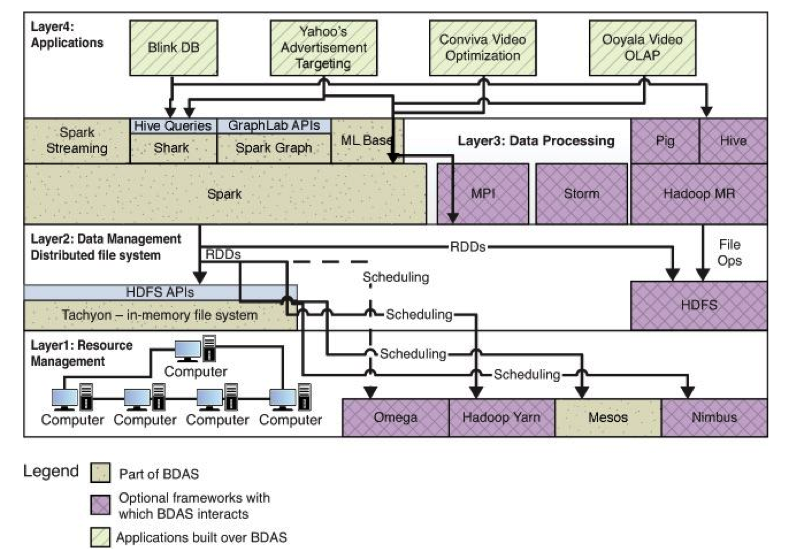
\includegraphics[width=1.0\textwidth]{bilder/2_2_stack.png}
\caption{Der BDAS. Abbildung aus „Big Data Analytics Beyond Hadoop“, S 15 \protect\citelit{va14}}
\label{fig:bdas]}
\end{figure} 


\section{Apache Mesos}
\label{section:apache Mesos}


Bei Apache Mesos handelt es sich um ein Cluster-Management-Framework für Anwendungen, die in verteilten Serverpools laufen sollen. Bestandteil von Mesos ist wiederum Apache ZooKeeper, das für Konfigurationsinformationen, Naming-Services und die Synchronisation von verteilten Anwendungen zuständig ist.  

Mesos wird im BDAS eingesetzt, um die Prozesse von Hadoop/Spark effizient auf die einzelnen Knoten im Cluster zu verteilen. Besonders das Ressourcen-Management und –Monitoring innerhalb des Clusters ist ein wichtiger Faktor, um Jobs performant auf verteilten Systemen ausführen zu können. Auch das Fehlerhandling für Knoten, Prozesse und im Netzwerk wird im Berkeley-Stack von Mesos übernommen. 

Ein besonderer Vorteil von Mesos gegenüber Yarn oder anderen Alternativen, wie dem Cloudera Cluster Manager oder Ambari von Hortonworks ist die Möglichkeit, verschiedene Frameworks gleichzeitig und isoliert in einem Cluster betreiben zu können. So kann beispielsweise Hadoop mit Spark in einer gemeinsamen Infrastruktur koexistieren.   
	
\section{Hadoop Distributed File System (HDFS) und Tachyon}
\label{section:hadoop Distributed File System (HDFS) und Tachyon}


Das Hadoop Distributed File System basiert ideologisch auf dem GoogleFileSystem (GFS) und hat zum Zweck, zuverlässig und fehlertolerant sehr große Dateien über verschiedene Maschinen hinweg in verteilten Umgebungen zu speichern. In entsprechenden Veröffentlichungen von Hortonworks \citeint{ho14} wird von Produktivsystemen berichtet, die bis zu 200 PetaByte an Datenvolumen in einem Cluster von 4500 Servern basierend auf HDFS verwalten.

HDFS wurde speziell für den Einsatz mit MapReduce entwickelt, ist also auf geringe Datenbewegungen ausgelegt, da MR die Berechnungsprozesse jeweils zu den physischen Datensätzen selbst bringt und nicht, wie herkömmlich, die Daten zu den Prozessen geliefert werden müssen. So wird massiv Netzwerkverkehr innerhalb des Clusters eingespart und letztlich werden nur Prozesse und Prozessergebnisse verschickt.  

Die Hauptbestandteile von HDFS sind der sogenannte NameNode, der die Metadaten des Clusters verwaltet und die DataNodes, die die eigentlichen Daten halten. Dateien und Verzeichnisse werden vom NameNode durch inodes repräsentiert. Diese wiederum enthalten Informationen über Zugriffsrechte, Zugriffszeiten oder Größenangaben der Dateien.



\begin{figure}[htb!] 
\centering
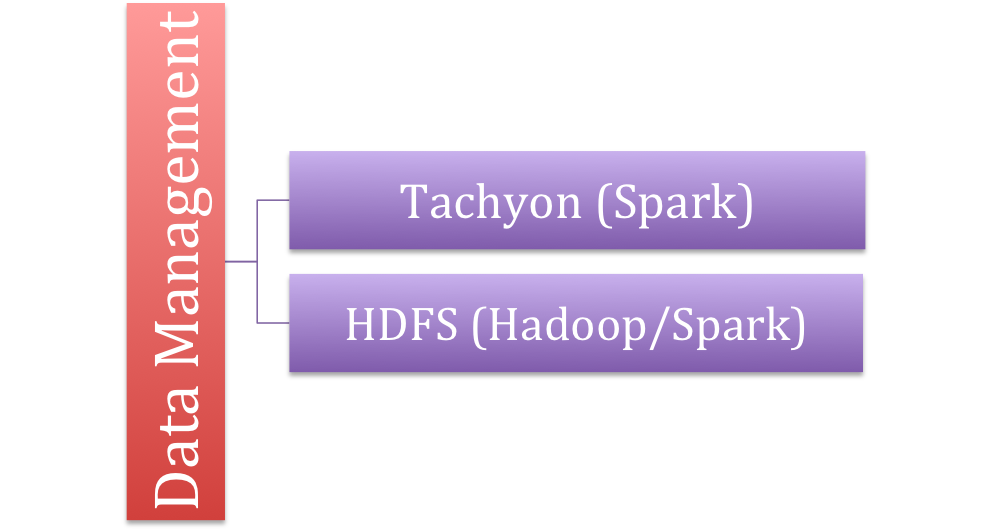
\includegraphics[width=1.0\textwidth]{bilder/2_3_stack.png}
\caption{Der Datamanagement-Layer im BDAS mit HDFS und Tachyon}
\label{fig:datamgmtlayer}
\end{figure} 

 

In Abbildung 2.3 wird die Datenmanagementschicht des BDAS nochmals detaillierter dargestellt. Hier ist erkennbar, dass reine Hadoop-Implementierungen direkt auf dem HDFS aufsetzen, da das HDFS für MapReduce optimiert ist. 

Kommt hingegen Spark zum Einsatz, lässt sich wahlweise direkt das HDFS ansprechen oder alternativ eine Zwischenschicht nutzen, die auf das In-Memory-Modell von Spark zugeschnitten ist. Dies ist innerhalb des BDAS das verteilte Dateisystem Tachyon. Hier werden die zu verarbeitenden oder zu analysierenden Datensätze direkt in den Hauptspeicher des jeweiligen Knoten gecached. Somit werden Lade- und Speicheroperationen auf Massenspeicher minimiert und eine massiv höhere Ausführungsgeschwindigkeit erreicht. Unterhalb von Tachyon ist nach wie vor ein HDFS für die persistente Datenhaltung notwendig. Alternativ kann auch das Amazon S3-File-Sytem eingesetzt werden. Tachyon wurde direkt innerhalb der AMPLabs entwickelt und ist mittlerweile fester Bestandteil des BDAS.  


\section{Apache Spark}
\label{section:apache Spark}

Spark ist das Herzstück des BDAS. Bei Spark handelt es sich um ein open-source Data-Analytics-Framework, das, wie Hadoop, speziell für die Bedürfnisse im Rechner-Cluster konzipiert ist. Auch Spark nutzt das HDFS entweder direkt, oder indirekt über Tachyon. Im Gegensatz zu Hadoop bietet Spark jedoch Funktionen für In-Memory-Cluster-Berechnungen und ist nicht zwingend an MapReduce gebunden. Besonders interaktive Analyse oder Verarbeitung der Daten, Abfragen über verteilte Dateien und iterative 

Lernalgorithmen erfahren so laut AMPLab eine bis zu hundertfache Ausführungs-geschwindigkeit im Gegensatz zu Hadoop. Auch die im ersten Kapitel angesprochenen Schwächen von Hadoop bei Berechnungen von komplexen linear-algebraischen Problemen, generalisierten n-Körper-Problemen, diversen Optimierungsproblemen und diversen anderen Aufgaben, treten bei Spark auf Grund der offenen Architektur und der Zerlegung von Datensätzen in die sogenannten Resilient Distributed Datasets (RDD) nicht mehr auf.

Spark wurde komplett in Scala entwickelt und bietet APIs für Scala, Java (inklusive Lambda-Expressions von Java 8) und Python. Im Labor existieren bereits Spark-Installationen mit bis zu 2000 Knoten, in Produktivsystemen sind bisher Systeme mit bis zu 1000 Knoten im Einsatz \citeint{cm13}. Durch die Möglichkeit, die Datensätze im Speicher für interaktive Analyseaufgaben zu cachen und iterativ abzufragen, ist eine direkte Kommandozeileninteraktion über das integrierte Scala REPL (alternativ auch in Python) möglich. 

Für Spark existieren dedizierte Bibliotheken für Verarbeitung von Datenströmen, Machine-Learning und Graphenverarbeitung. Ähnliche Artefakte existieren auch für Hadoop (Mahout, Vowpal Wabbit, etc.), jedoch ist die Architektur von Spark wesentlich besser für derartige Anwendungsbereiche zugeschnitten. 
   
\subsection{Spark Streaming}
\label{section:spark Streaming}


Spark Streaming ist eine der oben genannten Bibliotheken, die Spark um dedizierte Anwendungsbereich erweitert. Hierbei handelt es sich um eine Erweiterung, um die integrierte API von Spark für Anwendungen auf Datenströmen nutzen zu können. Das Programmiermodell unterscheidet nicht zwischen Batch- und Streaming-Anwendungen. So lassen sich beispielsweise Datenströme zur Laufzeit mit Archivdaten vergleichen und direkt Ad-hoc-Abfragen auf die Ströme formulieren. Im Fehlerfall ermöglicht Streaming zahlreiche Wiederherstellungsoptionen, sowohl von verlorenen Datenströmen, als auch von Einstellungen. Ein Anwendungsbeispiel ist die Echtzeitanalyse von Twitter-Meldungen. 

\subsection{GraphX}
\label{section:graphX}


GraphX ist eine Erweiterung für Spark, die verteilte, flexible Graphen-Anwendungen in einem Spark-Cluster ermöglicht \citeint{xg13}. Besonders in den Disziplinen „Machine Learning“ und „Data Mining“ ist die Anwendung komplexer Graphen unerlässlich. Graph-datenbanken kommen immer dann zum Einsatz, wenn stark vernetzte Informationen und ihre Beziehungen zueinander interessant sind. Hier werden die Entitäten als Knoten behandelt, die Beziehungsart definiert die Kanten. Die Kanten können auch gewichtet 

sein. Ein konkretes Beispiel sind die Mitglieder eines sozialen Netzwerks mit ihrem jeweiligen Beziehungsgeflecht. Je nach Kontaktintensität können diese Beziehungen auch priorisiert werden, was hier dem Kantengewicht entspricht.

GraphX nutzt hier die Vorteile der darunterliegenden Spark-Infrastruktur, in dem durch eine tabellarische Anordnung der Datenstrukturen eine massive Parallelisierung möglich ist und auch der Verarbeitung in RDDs voll unterstützt wird. So sind auch interaktive Operationen auf den Graphen jederzeit über REPL möglich. 

\subsection{MLbase/MLLib}
\label{section:mLbase/MLLib}


MLbase ist eine Sammlung von Bibliotheken und Werkzeugen für Machine-Learning-Anwendungen mit Spark. Sie besteht grundsätzlich aus den drei Teilen MLlib, MLI und ML-Optimizer und ist oberhalb der Spark-Installation angesiedelt, wie auf Abbildung 2.4.3. zu erkennen ist. 

\begin{figure}[htb!]
\centering
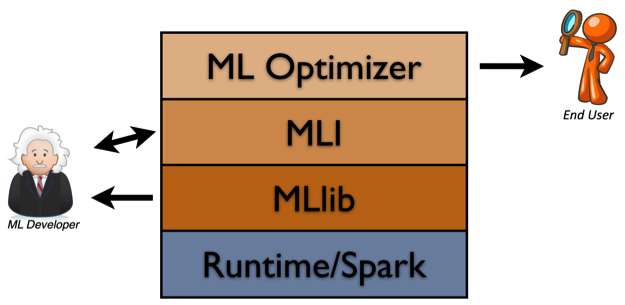
\includegraphics[width=1.0\textwidth]{bilder/2_4_3_mlbase.png}
\caption{Die Bestandteile der MLbase \protect\citeint{ml10}}
\label{fig:mlbase}
\end{figure} 
 


Die MLlib ist eine verteilte Machine-Learning-Bibliothek die für die Spark-Laufzeitumgebung entwickelt wurde und die bekannten Algorithmen für Probleme wie Klassifikation, Regression, Clustering und kollaboratives Filtern enthält.

Bei MLI handelt es sich um eine API, die es ermöglicht, selbst ML-Features zu entwickeln und in erster Linie für komplexere Problemstellungen geeignet ist. Mit MLI lassen sich die Funktionen direkt gegen Spark entwickeln, gegebenenfalls unter Zuhilfenahme der Bibliotheken der MLlib.

Der ML-Optimizer soll ML-Probleme für Endnutzer vereinfachen, in dem Modellauswahlen automatisiert werden. Hierzu werden Features aus der MLlib und der MLI extrahiert und zur Hilfe genommen.



\subsection{Shark}
\label{section:shark}



Hive ist eine SQL-Query-Engine für Hadoop, die sich großer Beliebtheit in der Hadoop-Community erfreut. Shark ist eine Portierung dieser Engine für Spark, um alle Vorteile der In-Memory-Architektur nutzen zu können und ist kompatibel mit sämtlichen Hive-Daten, -Metastores und –Queries. Im Gegensatz zu Hive, das aus Datensätzen zur Laufzeit Java-Objekte generiert, nutzt Shark eine zeilenorientierte Speicherung mittels Arrays primitiver Datentypen und ist somit selbst in einer Hadoop-Infrastruktur im Mittel bis zu fünfmal schneller als Hive. 

Eine Besonderheit von Shark ist neben seinem SQL-Interface die Möglichkeit, auch Machine-Learning-Funktionen als Abfragen formulieren zu können. 

Für die Anwendung von Shark hat sich die Architektur von Spark mit seinen RDDs als sehr vorteilhaft erwiesen, da Abfragen auf Fehlerhaften RDDs nach dem Neuaufbau des entsprechenden Datasets direkt erneut ausgeführt werden können. 

Ein weiterer Unterschied zu Hive ist die sogenannte Partial-DAG-Execution (PDE). Dies bedeutet, dass logische Abfragepläne in Shark aufgrund gesammelter Statistiken zur Laufzeit flexibel erstellt werden im Gegensatz zu Hive oder herkömmlichen relationalen Datenbanksystemen, wo bereits zur Kompilierungszeit starre physische Abfragepläne generiert werden. Besonders die Machine-Learning- und Failover-Funktionen wären mit einer Planerstellung zu Kompilierzeit nicht umsetzbar. 


\section{Alternative Wege innerhalb des BDAS}
\label{section:alternative Wege innerhalb des BDAS}


Wie in den Abbildungen 2.1 und 2.2 ersichtlich, existieren auf jeder Ebene des BDAS auch alternative Implementierungen. Einige davon werden im Folgenden kurz vorgestellt. 


\subsection{Hadoop MR (MapReduce)}
\label{section:hadoop MR (MapReduce)}


Alternativ zu Spark lässt sich im BDAS auch Hadoop als Kernimplementierung für die Datenanalyse oder -verarbeitung im Cluster einsetzen. Dies könnte beispielsweise sinnvoll sein, wenn die Infrastruktur des Clusters über relativ wenig Hauptspeicher verfügt, so dass Spark seinen In-Memory-Vorteil nicht ausspielen kann und die Aufgaben ohnehin den im ersten Kapitel beschriebenen einfachen statistischen Problemen entsprechen. 
 
Hadoop besteht in erster Linie aus dem Hadoop File System (HDFS) und dem MapReduce-Programmiermodell. Dieses wurde von Google speziell entwickelt, um große Datensätze parallel in Clustersystemen verarbeiten und generieren zu können. 

\begin{figure}[htb!]
\centering
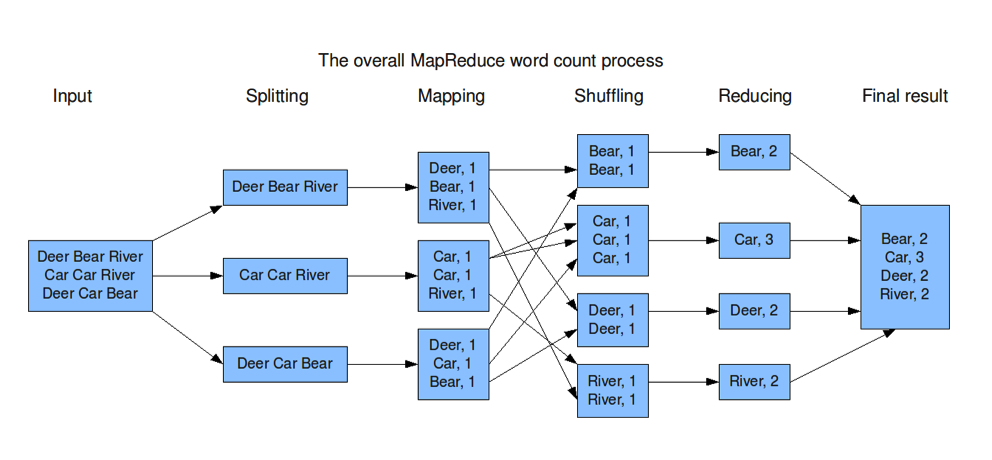
\includegraphics[width=1.0\textwidth]{bilder/2_6_1_wordcount.png}
\caption{Ein konkretes Word-Count-Beispiel für MapReduce  \protect\citeint{xi12}}
\label{fig:wordcount}
\end{figure}   
 


In Abbildung 2.6.1 wird das MapReduce-Modell an einem praktischen Beispiel zur Wortzählung gezeigt. Bei MapReduce wird zunächst eine problemspezifische Map-Funktion definiert. Diese splittet die Ursprungsmenge in gleichgroße Teile, versieht unstrukturierte Worte in einem ersten Schritt mit Standardwerten, um so aus jedem unstrukturierten Datensatz ein Key-Value-Pair zu generieren. Im gezeigten Beispiel wird hier jedem Wert eine Eins als Anzahl zugeordnet. Im nächsten Schritt werden diese so gewonnenen Zwischen-Key-Value-Paare in einem Shuffling-Prozess klassifiziert und die so homogenisierten Pakete auf die Knoten im Cluster verteilt. Nun enthält jede Ausführungseinheit nur noch gleiche Wörter. Im Reduce-Schritt schließlich, werden die gleichartigen Wörter zu Gesamtmengen zusammengefasst, addiert und im Endergebnis aggregiert. 

An dem gezeigten Beispiel lässt sich gut erkennen, dass die einzelnen Ausführungsschritte jeweils parallelisiert und auf separate Knoten im Cluster verteilt werden können. Das Laufzeitsystem kümmert sich um die Details der Partitionierung der Eingabedaten, die Ressourcenverwaltung innerhalb des Clusters, das Behandeln von Fehlern und die Kommunikation zwischen den einzelnen Knoten. 
 
\subsection{Hive}
\label{section:hive}


Apache Hive ist eine Data-Warehouse-Infrastruktur für Hadoop, die ursprünglich von Facebook entwickelt wurde. Hive ermöglicht die Analyse sehr großer Datensätze mittels einer SQL-ähnlichen Abfragesprache HiveQL, die volle Unterstützung für MapReduce-Verarbeitung bietet. 

Um Abfragen zu beschleunigen, nutzt die Query-Engine Datenbankindizes, die, zusammen mit Metadaten, in einer eigenen Apache Derby-Datenbank gespeichert werden.


Hive kann auf einer Hadoop-basierten Alternativinfrastruktur verhältnismäßig viel Leistung bieten. Wird jedoch Spark eingesetzt, sollte auf jeden Fall Shark statt Hive zum Einsatz kommen, wie in Kapitel 2.4.4 beschrieben.

\subsection{Storm}
\label{section:storm}


Storm ist, wie Apache Streaming, ein Framework für Hadoop, bzw. Spark für verteilte Streaming-Anwendungen. Wo Spark ganz klar eine Verbesserung gegenüber Hadoop darstellt und Shark dementsprechend für Hive, ist die Situation bei Storm und Apache Streaming dagegen nicht so klar determinierbar. 

Storm und Spark Streaming unterscheiden sich fundamental in ihren Verarbeitungsmodellen \citeint{va14}. Das erstgenannte Framework verarbeitet eintreffende Events nacheinander, immer genau eines pro Zeitraum. Spark Streaming sammelt im Gegensatz dazu die Events in Mini-Batch-Jobs und verarbeitet sie paketweise zu definierten Zeiträumen nach wenigen Sekunden. Deshalb kann Storm Latenzzeiten von deutlich unter einer Sekunde erreichen, während Spark Streaming eine Latenzzeit von einigen Sekunden aufweist. Diesen Nachteil macht Spark Streaming durch eine sehr gute Fehlertoleranz wett, da die Mini-Batches nach aufgetretenen Fehlern einfach nochmals bearbeitet werden können und die zuvor fehlerhaft ausgeführte Verarbeitung verworfen wird. Treten hingegen bei Storm Fehler auf, wird genau dieser Datensatz nochmals verarbeitet. Dies bedeutet, dass dieser auch mehrfach verarbeitet werden kann. Durch dieses Verhalten lassen sich die beiden Frameworks grob in zwei Einsatzgebiete verteilen:

Storm ist das Framework der Wahl, wenn Wert auf sehr kurze Latenzzeiten gelegt werden muss, hingegen ist es für statusbehaftete Anwendungen durch die Möglichkeit der Mehrfachverarbeitung ungeeignet. Im Umkehrschluss ist Spark Streaming eine gute Wahl, wenn aufgrund der gestreamten Daten eine Statusmaschine aufgebaut werden soll. Dafür müssen hier höhere Latenzzeiten in Kauf genommen werden.     




